\documentclass[main.tex]{subfiles}

%\externalcitedocument{bibfile}

\begin{document}


\section{Neutrinos: A Primer}
Neutrinos make up three of the seventeen known fundamental particles to exist in nature, shown in Figure~\ref{fig:party}
\begin{figure}
    \centering
    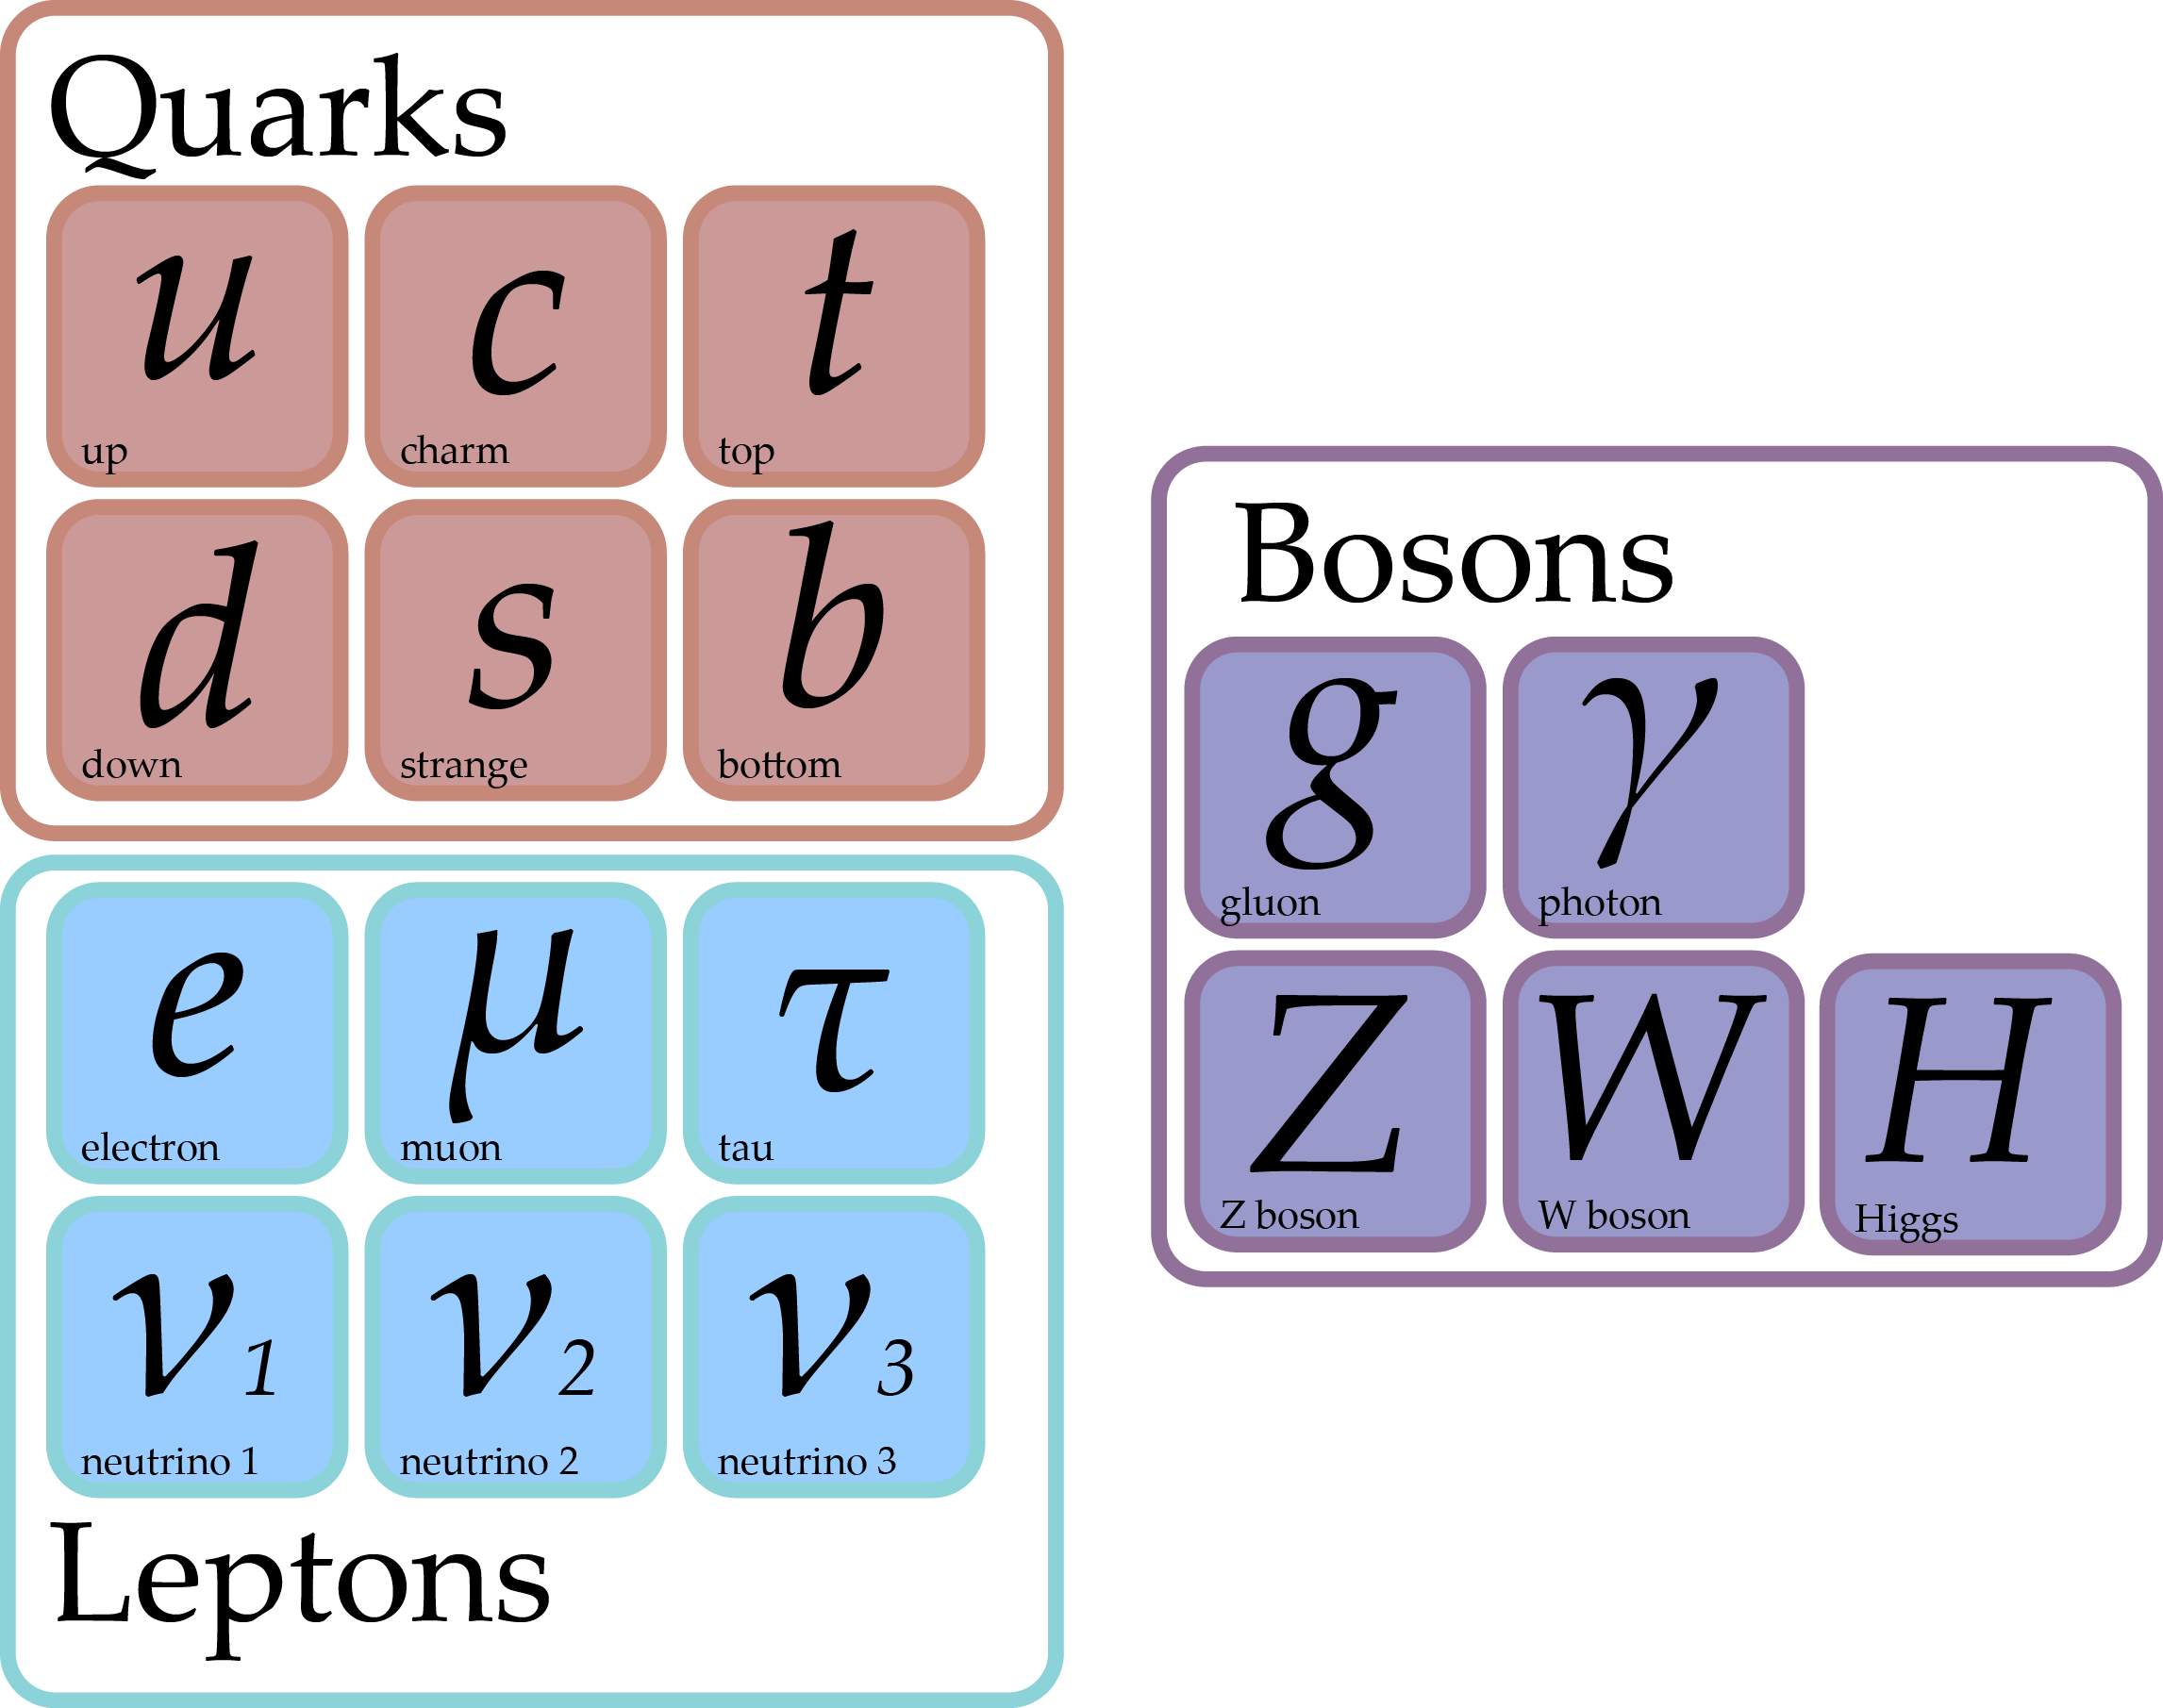
\includegraphics[width=0.8\linewidth]{figures/particles.png}
    \caption{A table of the seventeen fundamental particles. Only the mass-eigenstates for the fermions are shown.}\label{fig:party}
\end{figure}
The three-mass and three active-flavor neutrino \index{neutrino} paradigm has been well-studied~\cite{PhysRevD.98.030001,Esteban_2019,de_Salas_2018,Capozzi_2016,zboson2006, berns2021recent}, and is the conventional understanding.
At least two are known to be massive, but as of the time of writing there exist only upper bounds on their masses, and it is uncertain by which mechanism neutrinos get their mass.

However, several anomalies persist at short baselines, including in $\nu_\mu\rightarrow\nu_e $ appearance in decay-in-flight~\cite{aguilar2018significant} and decay-at-rest~\cite{Athanassopoulos_1998} beams  and $\nu_e\rightarrow\nu_e$ disappearance at reactors~\cite{mention2011reactor,serebrov2019first}  and with $^{71}$Ga electron capture sources~\cite{PhysRevC.73.045805,giunti2011statistical}.  
These anomalies have been attributed to possible oscillations of unknown neutrinos with mass-squared differences in the range of $\Delta m^{2}\sim 0.1-10\text{ eV}^{2}$~\cite{abazajian2012light}.   
Such an additional neutrino flavor state must be non-weakly interacting, or ``sterile,'' to be consistent with observed decay widths of the Z-boson~\cite{zboson2006}; the simplest such model is known as the ``3+1'' light sterile neutrino model in which a single sterile neutrino is added. 

There have been interesting recent developments for the 3+1 model.  
The BEST experiment appears to validate the anomalous electron neutrino disappearance signature of the previous gallium anomalies with a new level of statistical significance and experimental precision~\cite{barinov2021results}. 
The Neutrino-4 experiment claims evidence of short-baseline oscillations in the $\bar{\nu}_e$ disappearance channel with $\Delta m^2\sim 7.3\,\mathrm{eV}^2$ at the 2.9$\sigma$ level.
 Meanwhile results from the MicroBooNE~\cite{microboonecollaboration2021search,microboonecollaboration2021search1,microboonecollaboration2021searchmulti} experiment challenge the interpretation that the MiniBooNE low energy excess~\cite{miniboone2018} is due entirely to the electron neutrino by placing a constraint on the sterile neutrino interpretation of the excess; though the impact of this observation on the 3+1 model has yet to be assessed.  Continued exploration of sterile neutrino mixing in all channels and all energy ranges thus remains strongly motivated~\cite{sbnfermilab}.

The addition of a fourth neutrino mass and flavor eigenstate expands the unitary mixing matrix to four dimensions. 
The four-neutrino oscillations model becomes an extension of the three-neutrino model with three additional mixing angles $\theta_{14}$, $\theta_{24}$, and $\theta_{34}$, and two new CP-violating phases $\delta_{14}$ and $\delta_{24}$. These three new mixing angles parametrize the amplitude of oscillations between the three active states and the one sterile state, and lead to additional short-baseline vacuum-like oscillations as well as novel effects in the presence of matter~\cite{Akhmedov:1988kd,KRASTEV1989341,Chizhov:1998ug, Chizhov_1999, Akhmedov_2000, Nunokawa:2003ep,Petcov:2016iiu}.  In this work we consider CP-conserving models with all CP-violating phases set to zero.

Of particular interest to neutrino telescopes, matter effects can result in the near complete disappearance of TeV-scale muon anti-neutrinos passing through the Earth's core for a sterile neutrino with eV-scale mass squared differences~\cite{Nunokawa:2003ep, Choubey:2007ji, Barger:2011rc, Esmaili:2012nz, esmaili2013restricting, Lindner:2015iaa}. This signature of matter-enhanced resonant disappearance has been targeted by the IceCube Neutrino Observatory~\cite{Aartsen_2020, Aartsen_2020_prd}, leading to one of the  most sensitive $\nu_\mu$ disappearance analyses to date. The result of the analysis was a closed 90\% contour with best fit point at $\sin^2 2\theta_{24}\sim0.1$ and $\Delta m^2_{14}=4.5\text{ eV}^2$, under a conservative assumption (for the $\nu_\mu$ disappearance channel) that $\theta_{34}=\theta_{14}=0$. In addition to being a strong refutation, lower mass solutions consistent with the LSND~\cite{Athanassopoulos_1998} and MiniBooNE anomalies and constraints around 1~eV$^2$~\cite{kopp2013sterile, Cirelli:2004cz, abazajian2012light, Gariazzo:2017fdh, Dentler:2017tkw, Diaz:2019fwt}, a possible interpretation of this result is as a statistically weak hint of a disappearance signature around $\Delta m^2_{41}\sim4.5\text{ eV}^2$.  Further exploration of this region of parameter space  in other channels at neutrino telescopes is therefore strongly motivated. 

\subsection{Neutrino oscillations}
\index{neutrino!oscillations}

First, a review of how these oscillations happen is of merit. From the solar neurino problem CITE it is understood that neutrinos oscillate, and from that we understand they have mass. To understand \textit{why} that is the case we consider that the neutrinos mass and flavor eigenstates are not identical. That there is some unitary matrix, 
\begin{equation}
    U_{\text{PMNS}} = \left(\begin{array}{ccc} U_{e1} & U_{e2} & U_{e3} \\ U_{\mu 1} & U_{\mu 2} & U_{\mu 3} \\ U_{\tau 1} & U_{\tau 2} & U_{\tau 3} \end{array}\right)
\end{equation}
which allows for transformations from the mass basis to the flavor basis, such that
\begin{equation}
    \left(\begin{array}{ccc} \nu_{e} & \nu_{\mu} & \nu_{\tau} \end{array}\right)  = \left(\begin{array}{ccc} U_{e1} & U_{e2} & U_{e3} \\ U_{\mu 1} & U_{\mu 2} & U_{\mu 3} \\ U_{\tau 1} & U_{\tau 2} & U_{\tau 3} \end{array}\right) \left(\begin{array}{c} \nu_{1} \\ \nu_{2} \\ \nu_{3} \end{array}\right).
\end{equation}
where $\nu_{i}$, $i\in\left(1,2,3\right)$ is in the mass basis and $i\in\left(e,\mu\tau\right)$ is in the flavor basis. 
We can, in general then, express a stationary state in one basis in terms of the other basis:
\begin{equation}\label{eq:nunu}
    \ket{\nu_{e}} = U_{e1} \ket{\nu_{1}} + U_{e2} \ket{\nu_{2}} + U_{e3}\ket{\nu_{3}}.
\end{equation}
To consider a neutrino in-flight, we consider the time-dependent Schr\"odinger Equation
\begin{equation}
    i\dfrac{\partial}{\partial t} \ket{\nu_{i} (t)} = \bvec{H}_{\nu}\ket{\nu_{i}(t)},
\end{equation}
which can be solved with the stationary state solution 
\begin{equation}
    \ket{\nu_{i} (t)}  =  e^{-iEt} \ket{\nu_{i} (0)}.
\end{equation}
For neutrinos, we can expand out the energy term and simplify under the small-mass assumption. 
\begin{align}
    E_{i} &= \sqrt{p^{2}c^{2} + m_{i}^{2}c^{4}} \\
    &\approxeq pc + \dfrac{m_{i}^{2}c^{4}}{2E}
\end{align}
The stationary state solution then becomes, using $t=L/c$ and $c=1$ 
\begin{equation}
    \ket{\nu_{i} (t)}  =  e^{-ipt}e^{ -m_{i}^{2}L/2E}\ket{\nu_{i} (0)}
\end{equation}
and for the state described in Equation~\eqref{eq:nunu},

\begin{equation}
    \ket{\nu_{e}(t)} = \sum\limits_{i} U_{ei} e^{-ipt}e^{ -m_{i}^{2}L/2E}\ket{\nu_{i} (0)}
\end{equation}

Oscillations probabilities can be calculated by projecting the final considered state onto this propagated state


\begin{equation}
    \braket{\nu_{\mu} | \nu_{e}(t)} = e^{-ipt} \sum\limits_{i} U_{\mu i}^{*}U_{ei} e^{ -m_{i}^{2}L/2E}
\end{equation}
To calculate actual transmission probabilities, we need the conjugate squared of this, $P_{e\mu} = \left|\braket{\nu_{\mu}|\nu_{e}(t)}\right|^{2}$. While the phase term, $e^{-ipt}$, cancels we are left with 
\begin{equation}\begin{split}
P_{\mu e}&= \sum\limits_{i}\left[\left|U_{\mu i}\right|^{2}\left|U_{e i}\right|^{2} \right.\\
&\hspace{1cm} + 2\sum\limits_{i>j}U_{\mu i}^{*}U_{e i}U_{\mu j}U_{e j}^{*}\left.e^{-i\Delta m_{ij}^{2}L/2E} \right]
\end{split}\end{equation} 
Using the sinusoidal form of the exponential, we can write this in other components 
\begin{equation}\begin{split}
    P_{\mu e}&= \sum\limits_{i}\left[\left|U_{\mu i}\right|^{2}\left|U_{e i}\right|^{2} \right.\\
    &\hspace{1cm} -2\sum\limits_{i>j} \Re(U_{\mu i}^{*}U_{e i}U_{\mu j}U_{e j}^{*})\cos\left(\Delta m_{ij}^{2}L/2E \right) \\
    &\hspace{1cm} -2\sum\limits_{i>j}\Im(U_{\mu i}^{*}U_{e i}U_{\mu j}U_{e j}^{*})\sin\left(\Delta m_{ij}^{2}L/2E \right)
\end{split}\end{equation} 

From this we notice a few things. 
Neutrino oscillation probabilities are dependent not just on the mass of the neutrino eigenstates, but the differences of square of the masses. 
Through oscillations we can only measure the absolute of the difference of the masses, and so the ordering of the masses will be invisible to oscillations. 
This also suggests that, since oscillations have been observed, at minimum two of the neutrino masses must be non-zero. 
Oscillations will also depend on the energy $E$ of the neutrinos involved and the baseline $L$ over which they travel. \index{neutrino!baseline}


\subsection{Neutrino Interactions}
\index{neutrino!interactions}
Discuss neutrino interactions at medium to high energies. Deep Inelastic Scattering

\subsection{Matter Effects on Neutrion Oscillations}
\index{neutrino!matter effect}
Neutrinos propagating in the presence of matter will experience a coherent forward elastic scattering with electrons and nucleons in the medium through which they propagate. Although all three neutrinos can scatter via Z$^{0}$ boson exchange with nucleons only $\nu_{e}$ can scatter via the exchange of W$^{\pm}$ and Z$^{0}$ with electrons. 
The consequence of these interactions is that neutrinos behave as if they had slightly different masses, which are referred to as effective massses, and so their oscillations are impacted.  
Mathematically, in the two-neutrino case the total effective Hamiltonian governing the neutrino propagation is modified via the orgogonal matrix 
\begin{equation}
    U^{m} = \left( \begin{array}{cc} \cos\theta^{m} & \sin\theta^{m} \\ -\sin\theta^{m} & \cos\theta^{m} \end{array}\right) 
\end{equation}





\end{document}